\documentclass[12pt, a4paper]{article}
\usepackage{caption}
\usepackage{graphicx}
\usepackage{listings}
\usepackage{siunitx}
\usepackage{hyperref}
\def\checkmark{\tikz\fill[scale=0.4](0,.35) -- (.25,0) -- (1,.7) -- (.25,.15) -- cycle;}
\usepackage{tikz-network}
\hypersetup{
    colorlinks,
    citecolor=black,
    filecolor=black,
    linkcolor=black,
    urlcolor=black
}
\usepackage{amsmath, amsfonts, amssymb, amsthm}
\renewcommand{\thesubsubsection}{\thesubsection.\alph{subsubsection}}
\title{Algorithms and datastructures\\Exercises}
\date{2022}
\author{Kristoffer Klokker}
\begin{document}
	\maketitle
	\clearpage
	\tableofcontents
	\clearpage
		\setcounter{section}{4}
		\section{Uge}
			\subsection{For each function $f(n)$ and time $t$ in the following table, determine the alrgest size $n$ of a problem that can be solved in time $t$, assuming that the algorithm to solve the problem takes $f(n)$ 1 nanosecond}
				\begin{table}[h!]
					\begin{tabular}{|l|l|l|l|l|}
					\hline
							& 1s 			& 1hour			& 1year			& 1 centuray                              	\\ \hline
					$n$    		& $10^9$ 		& $6\cdot 10^{10}$	& $3.2\cdot 10^{16}$	& $3.2\cdot 10^{18}$ 		\\ \hline
					$n \log_2 n$	& $4\cdot 10^7$	& $10^9\frac{1}{\text{s}}\cdot 3600\text{s}=n\cdot \log_2(n)\rightarrow n=  9.8\cdot10^{10}$  & $6.4\cdot 10^{14}$ & $5.6\cdot 10^{16}$                            \\ \hline
					$n^2$      	& $31622$		& $1.8\cdot 10^6$		& $1.7\cdot 10^8$		& $1.8\cdot 10^9$			\\ \hline
					$n^3$       	& $10^3$		& $15326$			& $316010$			& $1.4\cdot 10^6$                       \\ \hline
					$2^n$       	& 30 			& $41.7$			& $54.8$			& $61.5$			           \\ \hline
					\end{tabular}
				\end{table}	
			\subsection{Show that in a puzzle where two peices is switched with $n$ pieces in all wrong positions, it requires at minimum of $n/2$ switches to solve the puzzle}
				For a puzzle with no correct positions in advance, the lowest amounts of move will be in the scenario where every piece's correct position has to piece of its current position. Which therefore will result in $n/2$ amounts of moves is needed.
			\subsection{Create a puzzle with 4 pieces, and find a sequence of switches, but where not every switch moves at least one piece to its correct position}
				\begin{table}[h!]
					\begin{tabular}{|l|l|}
					\hline
					4&1\\\hline
					2&3\\\hline
					\end{tabular}
				\end{table}	
				$4\rightarrow 2,3\rightarrow 2, 1\rightarrow 2$\\
				As seen here this method does no use the greedy method but it still use the same amount of moves.
			\subsection{Create an algorithm which can find cycles in a given puzzle}
				The algorithm takes a list, and creates a variable counter for the amount of cycles.\\
				It then goes through every entry, if the entry is not -1 then it calls a recursive function with the entry index and list.\\
				The list then check if the given entry is -1 if not then set the entry to -1 and then calls itself with the entries last index and the list.\\
				When the function returns it add 1 to the cycle.\\
				Then it returns the amount of cycles\\
				This algorithm will run at $O(2n)$ if the cycle is 1 and it then has to move every entry and go through the rest of the list. 
			\subsection{Use the algorithm implementation to calculate statistic over the amount of cycles in a 16 long permutation}
				\begin{figure}[h!]
					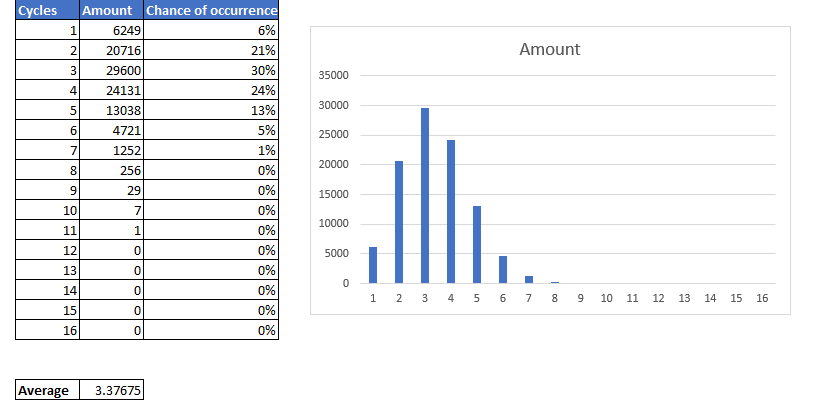
\includegraphics[width=\linewidth]{assets/week5Exercise2.png}
					\caption{Statistic from puzzleSolve/data.csv}
				\end{figure}
\end{document}


